\chapter{Iteration 4}
\label{ch:iter4}

This chapter documents the fourth iteration of HiringGuru, completed during the final phase of FYP-2. It focuses on the system design artifacts, detailing structural and behavioral aspects of the real-time mock interview platform. While the requirements analysis remains consistent across iterations, this phase emphasizes the design, development, and testing of HiringGuru’s architecture and components.

\section{Structural Design}

\subsection{Domain Model and Class Diagram}
The \textbf{Domain Model} outlines the conceptual structure of HiringGuru, defining core entities such as \texttt{User}, \texttt{Interview}, \texttt{AnalysisResults}, and \texttt{Feedback}, along with their relationships. For example, a \texttt{User} can participate in multiple \texttt{Interview} sessions, each generating \texttt{AnalysisResults} and \texttt{Feedback}. The \textbf{Class Diagram} provides a static view of the system, detailing classes like \texttt{UserProfile} (attributes: userID, email, name), \texttt{InterviewSession} (attributes: sessionID, timestamp, duration), and \texttt{AIAnalysis} (methods: analyzePosture(), detectExpression()). It illustrates associations between the Next.js frontend, Node.js backend, and AI analysis modules, ensuring a cohesive design.

\subsection{Component Diagram}
The \textbf{Component Diagram} depicts HiringGuru’s modular components: the Next.js frontend styled with TailwindCSS, the Node.js backend for business logic, AI analysis modules (MobileNetV2 for posture detection \cite{howard2018mobilenetv2}, MediaPipe for landmark tracking \cite{lugaresi2019mediapipe}, Haarcascade for facial expressions \cite{viola2001haar}, Dlib for eye tracking \cite{king2009dlib}), Python TTS for voice conversion, and Firebase for real-time data storage \cite{firebase2023docs}. It highlights interfaces and dependencies, such as the backend’s reliance on Firebase for user authentication and session data.

\subsection{Layer Diagram}
The \textbf{Layer Diagram} organizes HiringGuru into four distinct layers:
\begin{itemize}
    \item \textbf{Presentation Layer}: Next.js with TailwindCSS delivers a responsive user interface \cite{vercel2023nextjs}.
    \item \textbf{Business Logic Layer}: Node.js handles interview session management and API coordination.
    \item \textbf{AI Analysis Layer}: TensorFlow, MediaPipe, and OpenCV (CV2) process webcam input for real-time feedback.
    \item \textbf{Data Access Layer}: Firebase manages user data, session logs, and analysis results.
\end{itemize}
This layered architecture ensures scalability and maintainability by isolating responsibilities.

\subsection{Structure Chart}
The \textbf{Structure Chart} illustrates the hierarchical organization of HiringGuru’s modules, including the core interview system, OpenAI API for question generation \cite{openai2023api}, Python TTS for voice output, and AI analysis components (posture detection with 90\% accuracy, facial expression analysis, eye tracking). It maps the flow of control, showing function calls between modules, such as the backend invoking AI analysis during an interview session.

\section{Behavioral Design}

\subsection{Flow Diagram}
The \textbf{Flow Diagram} outlines the operational sequence of HiringGuru: user authentication via Firebase, interview setup, real-time AI analysis (posture, facial expressions, eye tracking), question generation using the OpenAI API, and feedback delivery. It emphasizes the seamless integration of AI modules to provide immediate, actionable insights during mock interviews.

\subsection{Data Flow Diagram (DFD)}
The \textbf{Data Flow Diagram (DFD)} models the flow of data within HiringGuru. Key processes include webcam input preprocessing (using CV2 for grayscaling), AI analysis (MobileNetV2 for posture, Haarcascade for facial expressions, Dlib for eye tracking), and storage in Firebase. External entities like users interact with the system, while data stores (Firebase database) manage session logs and analysis results.

\subsection{Data Dictionary}
The \textbf{Data Dictionary} defines HiringGuru’s data elements:
\begin{itemize}
    \item \texttt{User}: Attributes (userID: string, email: string, name: string).
    \item \texttt{Interview}: Attributes (sessionID: string, timestamp: datetime, duration: integer).
    \item \texttt{AnalysisResults}: Attributes (sessionID: string, postureScore: float, expressionData: string, eyeContactStats: float).
    \item \texttt{Feedback}: Attributes (feedbackID: string, sessionID: string, suggestions: string).
\end{itemize}
Each entry specifies data types, constraints, and relationships, ensuring clarity in data management.

\subsection{Activity Diagram}
The \textbf{Activity Diagram} models the workflow of a mock interview session, including user authentication, interview initialization, real-time analysis (posture, facial expressions, eye tracking), question delivery, and feedback generation. Decision nodes handle scenarios like posture correction prompts if MobileNetV2 detects improper alignment.

\subsection{State Machine Diagram}
The \textbf{State Machine Diagram} defines the states of an interview session: ``Idle'', ``Authenticating'', ``Analyzing Posture'', ``Detecting Facial Expressions'', ``Tracking Eye Contact'', ``Generating Questions'', and ``Providing Feedback''. Transitions occur based on events such as posture changes (detected by MobileNetV2 \cite{howard2018mobilenetv2}) or question delivery (via OpenAI API \cite{openai2023api}).

\subsection{Sequence Diagram}
The \textbf{Sequence Diagram} illustrates interactions during an interview session, showing message exchanges between the Next.js frontend, Node.js backend, AI analysis modules (TensorFlow, MediaPipe, CV2, Dlib), OpenAI API, and Firebase database. It details the sequence of operations, such as initiating an interview, processing webcam input, and storing results.

\subsection{Interaction Overview Diagram}
The \textbf{Interaction Overview Diagram} provides a high-level view of HiringGuru’s interactions, combining elements of sequence and activity diagrams. It focuses on coordination between AI analysis modules and core components, ensuring efficient data flow and feedback delivery.

\section{Schema Design: ER Diagram}
The \textbf{Entity-Relationship (ER) Diagram} models HiringGuru’s Firebase database structure, defining entities like \texttt{Users} (attributes: userID, email, name), \texttt{Interviews} (attributes: sessionID, userID, timestamp), \texttt{AnalysisResults} (attributes: sessionID, postureScore, expressionData, eyeContactStats), and \texttt{Feedback} (attributes: feedbackID, sessionID, suggestions). Relationships include a one-to-many mapping between \texttt{Users} and \texttt{Interviews}, ensuring efficient data retrieval.

\section{Data Structure Design}
The \textbf{Data Structure Design} outlines data organization in HiringGuru: arrays store real-time posture and expression analysis results, JSON objects manage user profiles and interview sessions, and Firebase-optimized structures enable fast queries for session logs and feedback. This design ensures efficient storage and retrieval of AI-generated data.

\section{Algorithm Design}
This section details the key algorithms in HiringGuru:
\begin{itemize}
    \item \textbf{MobileNetV2}: Performs real-time posture detection with 90\% accuracy \cite{howard2018mobilenetv2}.
    \item \textbf{MediaPipe}: Provides lightweight, high-precision landmark tracking for enhanced posture detection \cite{lugaresi2019mediapipe}.
    \item \textbf{Haarcascade}: Detects facial expressions using pre-trained cascades \cite{viola2001haar}.
    \item \textbf{Dlib}: Tracks eye contact via facial landmark detection \cite{king2009dlib}.
    \item \textbf{OpenAI API}: Generates contextually relevant interview questions based on user profiles \cite{openai2023api}.
\end{itemize}
These algorithms are optimized for low-latency performance and integrated into HiringGuru’s AI analysis pipeline.

\section{Development Phase}
This phase enforces coding standards across HiringGuru’s components, including camelCase for variables (e.g., \texttt{userProfile}), PascalCase for classes (e.g., \texttt{AIAnalysis}), and inline comments for clarity. Static analysis tools like ESLint (for JavaScript) and Pylint (for Python) ensure code quality in the Next.js frontend, Node.js backend, and AI modules.

\subsection{Unit Testing}
Unit tests validate individual components of HiringGuru, ensuring reliability:

\begin{table}[!htbp]
\centering
\begin{tabular}{|c|p{6cm}|c|}
\hline
\textbf{Test Case ID} & \textbf{Description} & \textbf{Expected Output} \\
\hline
UT-01 & Verify posture detection with MobileNetV2 & Correct posture score returned \\
\hline
UT-02 & Test facial expression detection with Haarcascade & Accurate expression classification \\
\hline
UT-03 & Validate eye tracking with Dlib & Correct eye contact statistics \\
\hline
UT-04 & Ensure OpenAI API generates relevant questions & Contextually appropriate questions returned \\
\hline
\end{tabular}
\caption{Unit Test Cases for Iteration 4}
\label{tab:unit-test-cases}
\end{table}

\subsection{Test Suites}
Test suites encompass functional testing (e.g., interview workflow), integration testing (e.g., coordination between AI modules and backend), and regression testing after updates. Test cases address edge scenarios, such as low-light conditions affecting webcam input or errors in question generation.

\section{Maintainable Phase}

\subsection{CI/CD Pipeline}
\textbf{Continuous Integration and Continuous Deployment (CI/CD)} is implemented using GitHub Actions, automating unit and integration tests on code commits and deploying updates to the production environment. This ensures rapid iteration and high code quality throughout development.

\subsection{Deployment Diagram}
The \textbf{Deployment Diagram} illustrates HiringGuru’s infrastructure: Node.js servers are hosted on a cloud platform, Firebase provides real-time database and authentication services \cite{firebase2023docs}, TensorFlow models are deployed on edge devices for efficient AI analysis, and the Next.js frontend is served via a CDN for low-latency access.

\subsection{System-Level Testing}
System-level tests validate HiringGuru’s end-to-end functionality:

\begin{table}[!htbp]
\centering
\begin{tabular}{|c|p{6cm}|c|}
\hline
\textbf{Test Case ID} & \textbf{Description} & \textbf{Expected Output} \\
\hline
ST-01 & Verify end-to-end interview session workflow & User completes session with feedback \\
\hline
ST-02 & Ensure real-time analysis under varying network conditions & Analysis results remain accurate \\
\hline
ST-03 & Validate Firebase data consistency after session & All session data stored correctly \\
\hline
ST-04 & Test system scalability with 100 concurrent users & System handles load without crashes \\
\hline
\end{tabular}
\caption{System-Level Test Cases for Iteration 4}
\label{tab:system-test-cases}
\end{table}

\subsection{Version Control }
Version control is managed via \textbf{GitHub}, facilitating collaboration and change tracking across HiringGuru’s components. Access at: \url{https://github.com/12Samad/FYP-HiringGuru}.

\subsection{Configuration and Setup Manual (Optional)}
This section outlines setup instructions for HiringGuru:
\begin{itemize}
    \item \textbf{Dependencies}: Install Node.js, Next.js, TensorFlow, MediaPipe, OpenCV, and Dlib.
    \item \textbf{API Configuration}: Set up OpenAI API keys for question generation \cite{openai2023api}.
    \item \textbf{Database}: Configure Firebase for authentication and real-time database \cite{firebase2023docs}.
    \item \textbf{Deployment}: Deploy the Next.js frontend via a CDN and Node.js backend on a cloud platform.
\end{itemize}
A tool manual covers usage of development tools like VS Code, ESLint, and GitHub Actions.

\section{UML Use Case Diagram}
\begin{figure}[h]
  \centering
  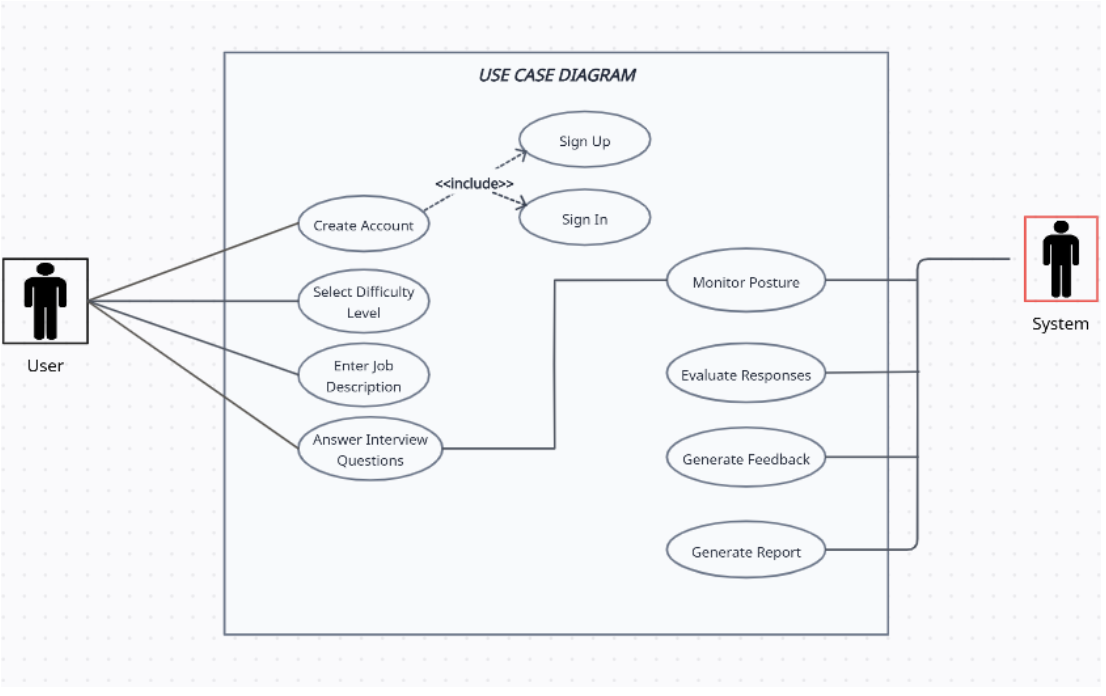
\includegraphics[width=0.8\textwidth]{sections/diagrams/UseCase.png}
  \caption{UML Use Case Diagram for HiringGuru}
  \label{fig:use-case}
\end{figure}

This chapter provides a comprehensive overview of Iteration 4, detailing the design, development, and testing of HiringGuru. The artifacts ensure a robust, maintainable platform with advanced AI-driven feedback capabilities for real-time mock interviews.